\documentclass{beamer}

%%%%%%%%%%%%%%%%%%%%%%%%%%%%%%%%%%%%%%%%%%%%%%%%%%%%%%%%%%%%%%%%%%%%%
%%	CONFIG
%%%%%%%%%%%%%%%%%%%%%%%%%%%%%%%%%%%%%%%%%%%%%%%%%%%%%%%%%%%%%%%%%%%%%

\usepackage[english]{babel}
\usepackage[utf8]{inputenc}
\usepackage{ucr_eie}
\usepackage{hyperref,url}
\usepackage{mdframed}
\usepackage{tikz}
\usepackage{chronology}
\usepackage{listings}
\usepackage{graphicx}
\DeclareGraphicsExtensions{.pdf,.png,.jpg}
\graphicspath{{../multimedia/imagenes}}
\definecolor{shadecolor}{RGB}{250,250,250}
\usetikzlibrary{arrows,positioning}
\addtobeamertemplate{background canvas}{\transduration{2}}{}
\lstset{
	basicstyle=\ttfamily,
	keywordstyle=\color{black},
	commentstyle=\color{black},
	stringstyle=\color{black},
	tabsize=2,
	backgroundcolor=\color{shadecolor}
	}

\title[dataCV]{
		dataCV: Library for data computing visualization.
		} 

\author[Campos, Apú, Soto]{
		Jose Carlos Campos Valerio\\
		Jose Pablo Apú Picado\\
		Jorge Soto Avendaño\\
		\medskip
		}

\institute[University of Costa Rica]{
		Electrical Engineering School \\
		IE-0217 - Estructuras de datos y algorítmos para ingeniería
		}

\date[\today]{
		1st Project \\
		\today
		}

%%%%%%%%%%%%%%%%%%%%%%%%%%%%%%%%%%%%%%%%%%%%%%%%%%%%%%%%%%%%%%%%%%%%%
%%	DOCUMENT
%%%%%%%%%%%%%%%%%%%%%%%%%%%%%%%%%%%%%%%%%%%%%%%%%%%%%%%%%%%%%%%%%%%%%

\begin{document}

\begin{frame}
  \titlepage
\end{frame}
%%%%%%%%%%%%%%%%%%%%%%%%%%%%%%%%%%%%%%%%%%%%%%%%%%%%%%%%%%%%%%%%%%%%%
\begin{frame}
  \frametitle{Outline}
  \tableofcontents
\end{frame}
%%%%%%%%%%%%%%%%%%%%%%%%%%%%%%%%%%%%%%%%%%%%%%%%%%%%%%%%%%%%%%%%%%%%%
\section{Introduction}
\begin{frame}
\frametitle{mysql++}
%% importancia del manejo de datos, utilizando bases de datos
\begin{center}
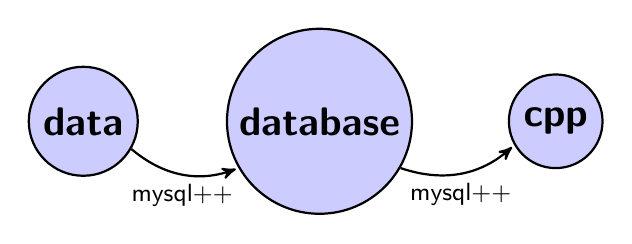
\begin{tikzpicture}[->,>=stealth',shorten >=1pt,auto,node distance=3cm,
  thick,main node/.style={circle,fill=blue!20,draw,font=\sffamily\Large\bfseries}]

  \node[main node] (1) {data};
  \node[main node] (2) [right of=1] {database};
  \node[main node] (3) [right of=2] {cpp};

  \path[every node/.style={font=\sffamily\small}]
    (1) edge [bend right] node[below] {mysql++} (2)
    (2) edge [bend right] node[below] {mysql++} (3);
\end{tikzpicture}
\end{center}
\end{frame}

\begin{frame}
\frametitle{gnuplot-cpp}

\end{frame}

\begin{frame}
\frametitle{mysqplot}
\end{frame}
%%%%%%%%%%%%%%%%%%%%%%%%%%%%%%%%%%%%%%%%%%%%%%%%%%%%%%%%%%%%%%%%%%%%%
\section{Body1}
\begin{frame}
\frametitle{mean - variance - standard deviation}
\end{frame}
%%%%%%%%%%%%%%%%%%%%%%%%%%%%%%%%%%%%%%%%%%%%%%%%%%%%%%%%%%%%%%%%%%%%%
\section{Plots}
\begin{frame}
\frametitle{histogram}
\end{frame}

\begin{frame}
\frametitle{gaussian distribution}
\end{frame}

\begin{frame}
\frametitle{scatterplot}
\end{frame}

\begin{frame}
\frametitle{jitterplot}

\begin{columns}

\begin{column}{0.3\textwidth}
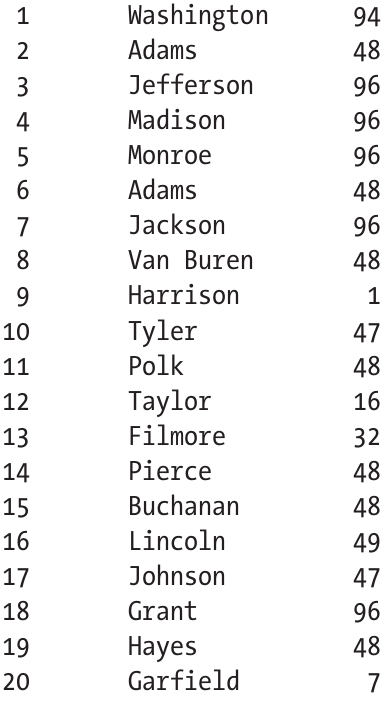
\includegraphics[scale=0.2]{jittertable}
\end{column}

\begin{column}{0.7\textwidth}
\begin{center}
gitterplot(meses,0);\\
gitterplot(meses,2);
\end{center}
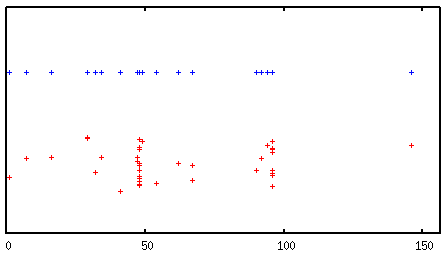
\includegraphics[scale=0.5]{jitterplot}

\end{column}
\end{columns}

\end{frame}

\begin{frame}
\frametitle{kde}
\end{frame}

\begin{frame}
\frametitle{pdf}
\end{frame}

\begin{frame}
\frametitle{cdf}
\end{frame}

%%%%%%%%%%%%%%%%%%%%%%%%%%%%%%%%%%%%%%%%%%%%%%%%%%%%%%%%%%%%%%%%%%%%%
\section{Body3}
\begin{frame}
\frametitle{Frame 1}
\end{frame}
%%%%%%%%%%%%%%%%%%%%%%%%%%%%%%%%%%%%%%%%%%%%%%%%%%%%%%%%%%%%%%%%%%%%%
\section{Conclusion}
\begin{frame}
\frametitle{Frame 1}
\end{frame}

\begin{frame}
\frametitle{Questions?}
\end{frame}
%%%%%%%%%%%%%%%%%%%%%%%%%%%%%%%%%%%%%%%%%%%%%%%%%%%%%%%%%%%%%%%%%%%%%
\end{document}
